\section{FASE 2. PRUEBAS DE SOFTWARE, TÉCNICAS DE TESTING Y REFACTORIZACIÓN}

\subsection{Pruebas de software aplicadas}
\label{subsec:testing}

Las pruebas de software aportan evidencia observable sobre si una operación responde conforme a los resultados esperados para entradas y estados determinados. En Tech-Flow son especialmente útiles para comprobar las reglas de venta, stock, importación y persistencia, cuya interacción afecta varios registros. Las pruebas existentes se implementan con JUnit Jupiter 5.10.0 y se ejecutan mediante Maven Surefire 3.2.5.

La suite está organizada en 16 clases de prueba y cubre clases de interfaz/control, modelos, servicios y dominio. Entre ellas se encuentran pruebas para \texttt{MotorCSV}, \texttt{IntegridadCSV}, \texttt{Verificador}, \texttt{Almacen}, \texttt{Vendedor}, \texttt{Gestor}, \texttt{Empleado}, \texttt{Producto}, \texttt{Proveedor}, \texttt{Inventario}, \texttt{Cliente}, \texttt{Rol}, \texttt{Main} y filtros de categorías. Varias clases utilizan \texttt{@TempDir} para aislar los archivos de prueba y evitar modificar los CSV ordinarios.

La ejecución registrada para el estado revisado fue \texttt{mvn -f Tech-Flow\textbackslash pom.xml test}, desde la carpeta que contiene \texttt{Tech-Flow}. El resultado fue \textbf{516 pruebas, 0 fallos, 0 errores y 0 omitidas}. Esta cifra es el resultado de esa ejecución documentada; no representa cobertura de código ni demuestra que todas las combinaciones posibles estén verificadas.
El 25 de noviembre de 2026 se ejecutaron nuevamente
las pruebas mediante el comando \texttt{mvn test},
obteniendo un total de 516 pruebas aprobadas, sin
fallos, errores ni pruebas omitidas.

\begin{figure}[H]
    \centering
    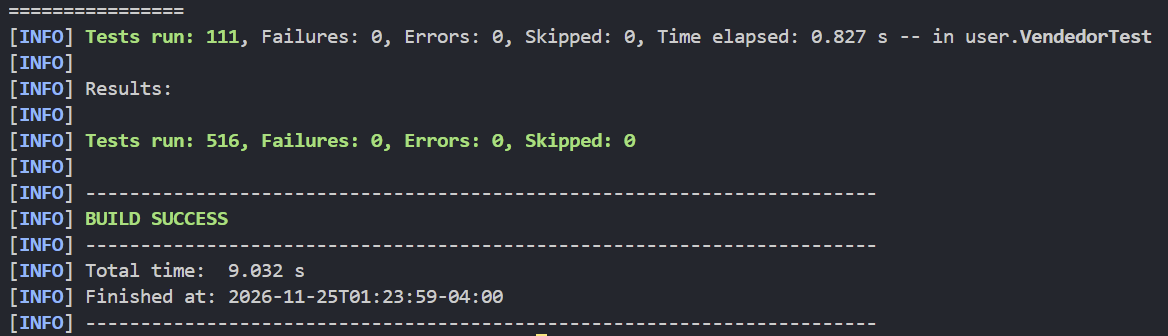
\includegraphics[width=\textwidth]{../capturas/pruebas-junit.png}
    \caption{Resultado de la ejecución de pruebas con JUnit y Maven.}
    \label{fig:pruebas-junit}
\end{figure}
\subsubsection{Configuración del entorno de pruebas}

El \texttt{pom.xml} declara \texttt{org.junit.jupiter:junit-jupiter:5.10.0} con alcance \texttt{test}, Maven Compiler Plugin 3.11.0 con fuente/destino Java 17 y Maven Surefire 3.2.5. Las pruebas siguen convenciones JUnit 5 como \texttt{@Test}, aserciones y, en casos de persistencia, directorios temporales. No se encontró una configuración para pruebas automatizadas de interfaz con TestFX, Selenium, Playwright u otra herramienta equivalente.

Las pruebas unitarias se enfocan en una clase u operación con datos aislados; las pruebas de integración observables verifican colaboraciones dentro del proceso, por ejemplo, cambios de inventario y registros CSV producidos por una venta. Una prueba funcional de extremo a extremo desde la GUI requeriría iniciar la aplicación, interactuar con controles y verificar el resultado visible y persistido. La suite disponible no equivale a esa automatización de extremo a extremo.

\subsubsection{Casos de prueba implementados}

La siguiente selección identifica métodos existentes. Todos los resultados mostrados como aprobados corresponden a la ejecución de la suite indicada; las entradas y expectativas se resumen desde el propósito y las aserciones de cada prueba.

\small
\begin{longtable}{|p{1cm}|p{3.4cm}|p{3.4cm}|p{3.1cm}|p{2.1cm}|}
\caption{Selección de pruebas automatizadas implementadas.}
\label{tab:casos-prueba}\\
\hline
\textbf{ID} & \textbf{Clase / método} & \textbf{Entrada o condición} & \textbf{Resultado esperado} & \textbf{Resultado}\\
\hline
\endfirsthead
\hline
\textbf{ID} & \textbf{Clase / método} & \textbf{Entrada o condición} & \textbf{Resultado esperado} & \textbf{Resultado}\\
\hline
\endhead
UT-01 & \texttt{MotorCSVTest}\newline\texttt{campoComplejo} & Campos con caracteres especiales. & Leer lo escrito preservando los campos. & Aprobado\\
\hline
UT-02 & \texttt{MotorCSVTest}\newline\texttt{campoCon\allowbreak SaltoDe\allowbreak Linea} & Valor con salto de línea dentro de comillas. & Recuperar el valor como una celda, no como dos filas. & Aprobado\\
\hline
UT-03 & \texttt{MotorCSVTest}\newline\texttt{actualizarFila\allowbreak Modifica} & Índice válido y nueva fila. & Persistir el reemplazo en el archivo. & Aprobado\\
\hline
UT-04 & \texttt{VerificadorTest}\newline\texttt{credenciales\allowbreak Correctas} & Usuario y contraseña existentes. & Aceptar credenciales y devolver el rol previsto. & Aprobado\\
\hline
UT-05 & \texttt{VerificadorTest}\newline\texttt{contrasena\allowbreak Incorrecta} & Usuario existente y contraseña distinta. & Rechazar autenticación. & Aprobado\\
\hline
UT-06 & \texttt{AlmacenTest}\newline\texttt{rechazaEntrada\allowbreak ConProveedor\allowbreak Inexistente} & Entrada referida a proveedor ausente. & Rechazar la operación sin aceptarla como entrada válida. & Aprobado\\
\hline
UT-07 & \texttt{AlmacenTest}\newline\texttt{importarCon\allowbreak Columnas\allowbreak Reordenadas\allowbreak DevuelveTrue} & Archivo con columnas reconocidas aunque cambie su orden. & Importar correctamente según los encabezados. & Aprobado\\
\hline
UT-08 & \texttt{VendedorTest}\newline\texttt{proformaNo\allowbreak DescuentaStock} & Preparación de una proforma. & Mantener el stock sin cambio antes de confirmar. & Aprobado\\
\hline
UT-09 & \texttt{VendedorTest}\newline\texttt{venderProducto\allowbreak Confirmado\allowbreak DescuentaStock} & Venta confirmada con unidades disponibles. & Registrar la venta y descontar la cantidad vendida. & Aprobado\\
\hline
UT-10 & \texttt{VendedorTest}\newline\texttt{noVendeConCaja\allowbreak Cerrada} & Intento de venta con caja cerrada. & Impedir confirmar la venta. & Aprobado\\
\hline
UT-11 & \texttt{VendedorTest}\newline\texttt{garantia\allowbreak Tiene\allowbreak Fecha\allowbreak FinDoce\allowbreak Meses} & Venta confirmada que genera garantía. & La fecha final refleja doce meses de vigencia. & Aprobado\\
\hline
UT-12 & \texttt{Integridad\allowbreak CSVTest}\newline\texttt{ventaConfirmada\allowbreak NoTiene\allowbreak ColumnasVacias} & Fila generada por venta confirmada. & Mantener completa la estructura esperada de la fila. & Aprobado\\
\hline
\end{longtable}
\normalsize

Una prueba de dominio comprueba explícitamente la diferencia entre crear una proforma y confirmar la venta:

\begin{lstlisting}[language=Java,caption={Prueba unitaria: una proforma no descuenta existencias.},label={lst:test-proforma}]
@Test
void proformaNoDescuentaStock() {
    Vendedor vendedor = vendedor();
    vendedor.generarOrdenDeVenta("Cliente", Map.of("P1", 2));
    assertEquals(10, vendedor.buscarEnInventario("P1").getStock());
}
\end{lstlisting}

La aserción valida el stock después de crear la proforma. El caso no sustituye las pruebas que comprueban el descuento tras confirmar la venta y se ejecuta con el aislamiento de datos configurado en la clase de prueba.

Esta selección es representativa y no pretende enumerar las 516 pruebas ejecutadas ni todos los casos de la suite. La tabla distingue condiciones probadas de evidencia visual: una captura de pantalla acredita que una vista se representó en cierto estado, pero no sustituye las aserciones ni prueba por sí sola el flujo completo.

\subsubsection{TDD: Red, Green, Refactor}

El desarrollo guiado por pruebas (Test-Driven Development, TDD) propone el ciclo \textbf{Red--Green--Refactor}: primero se redacta una prueba que falla porque el comportamiento aún no existe; después se implementa el cambio mínimo que la hace pasar; finalmente se refactoriza manteniendo la suite en verde. El ciclo ayuda a hacer explícito el comportamiento esperado y proporciona una red de regresión durante la mejora del diseño.

En el repositorio hay pruebas adecuadas para verificar comportamientos de dominio y persistencia, pero no se halló evidencia histórica suficiente para afirmar que el proyecto completo se construyera siguiendo TDD de manera estricta. La existencia de pruebas y el registro de correcciones no demuestran por sí solos el orden temporal Red--Green--Refactor. Por tanto, este informe explica el método y describe la cobertura disponible, pero no atribuye formalmente esa metodología a todo el proceso.

\paragraph{Pruebas durante el desarrollo del sistema.}

Durante el desarrollo de Tech-Flow se incorporaron
pruebas unitarias y se ampliaron los casos de validación
de manera progresiva.

El historial de versiones registra la implementación
de la clase Venta junto con sus pruebas en el commit
\texttt{cdb2d4c} del 12 de septiembre de 2026.

Posteriormente, en el commit \texttt{a91551f} del
3 de noviembre de 2026, se incorporaron pruebas
adicionales para la validación de datos y la
integridad de los archivos CSV.

Estas pruebas constituyen una base para verificar
el comportamiento del sistema durante las
correcciones y refactorizaciones posteriores.

\subsection{Bad Smells y refactorización}
\label{subsec:bad-smells}

Un Bad Smell es una señal de que una estructura puede dificultar el cambio, la comprensión o la prueba del software. No implica automáticamente un fallo funcional. En esta sección se separan problemas aún presentes de refactorizaciones con evidencia histórica; no se atribuye una mejora al proyecto si solo se observa la situación actual.


\paragraph{Bad Smell identificado: código duplicado (Duplicated Code).}

\textbf{Clase afectada:} \texttt{Main.java}.

\textbf{Situación inicial:} la aplicación de consola
utilizaba métodos propios para validar los nombres y
datos de los clientes, mientras que la interfaz gráfica
utilizaba la clase compartida \texttt{ValidadorDatos}.

\begin{lstlisting}[language=Java,caption={Validación antes de la refactorización.}]
private static boolean textoValido(String texto) {
    return texto != null && texto.matches(".*\\p{L}.*")
            && texto.matches("[\\p{L} ]+");
}
\end{lstlisting}

\textbf{Refactorización aplicada:} se eliminaron los
métodos locales de validación y se delegó esta
responsabilidad a la clase \texttt{ValidadorDatos}.

\begin{lstlisting}[language=Java,caption={Validación después de la refactorización.}]
if (!ValidadorDatos.textoValido(cliente)) {
    System.out.println("El nombre del cliente es obligatorio.");
    return;
}
\end{lstlisting}

\textbf{Beneficios:} se reduce la duplicación de código,
se facilita el mantenimiento y se unifican los criterios
de validación entre la consola y la interfaz gráfica.

La modificación también permitió aceptar nombres
alfanuméricos, por lo que se actualizaron los casos de
prueba correspondientes.

\textbf{Verificación:} las 516 pruebas automatizadas
aprobaron en la ejecución del 25 de noviembre de 2026.

\textbf{Referencia:} commit \texttt{a618180} del
18 de noviembre de 2026, registrado en el historial Git
del proyecto.

\paragraph{Bad Smell identificado: responsabilidades mezcladas en controladores.}
\textbf{Clase o método afectado:} \texttt{AdminController}, \texttt{VendedorController} y \texttt{AlmacenController}.

\textbf{Situación inicial:} los controladores gestionan eventos y componentes gráficos, y algunos también realizan lecturas directas de CSV o contienen lógica de presentación de informes. El diseño actual conserva estas responsabilidades en más de un lugar; no existe una capa DAO/repositorio tipada que medie todos los accesos.

\textbf{Consecuencias:} el acoplamiento entre JavaFX y el formato/índice de columnas dificulta probar la interfaz separadamente, modificar el esquema CSV y reutilizar las consultas.

\textbf{Refactorización aplicada:} se extrajeron utilidades compartidas para presentación, selección/escritura de archivos de informes y nombres de CSV, entre ellas \texttt{AyudasUI}, \texttt{InformeTexto}, \texttt{AyudasArchivo} y \texttt{ArchivosCSV}. La extracción reduce duplicación concreta, pero no elimina todo acceso directo desde controladores.

\textbf{Situación posterior y beneficios:} determinadas operaciones repetidas cuentan con puntos compartidos y los nombres de archivos se centralizan. La separación sigue siendo parcial; no se afirma una arquitectura por capas estricta.

\textbf{Verificación:} las pruebas de regresión del estado actual pasan en la ejecución registrada. Esto comprueba comportamientos cubiertos, no la eliminación completa del acoplamiento.


\paragraph{Refactorización mediante extracción de métodos compartidos.}

\textbf{Clases afectadas:} \texttt{AdminController} y
\texttt{VendedorController}.

\textbf{Bad Smell:} código duplicado (Duplicated Code).

\textbf{Situación inicial:} los controladores repetían
las instrucciones necesarias para seleccionar una ruta,
comprobar la extensión del archivo y guardar informes,
ventas y proformas en formato TXT.

\begin{lstlisting}[language=Java,caption={Selección de archivo antes de la refactorización.}]
FileChooser selector = new FileChooser();
selector.setTitle("Guardar venta");
selector.setInitialFileName("venta-" + idOrden + ".txt");
selector.getExtensionFilters().add(
    new FileChooser.ExtensionFilter(
        "Archivo de texto (*.txt)", "*.txt"));
java.io.File archivo =
    selector.showSaveDialog(Navegador.ventana());
if (archivo == null) {
    return;
}
\end{lstlisting}

\textbf{Refactorización aplicada:} se creó la clase
\texttt{AyudasArchivo}, que centraliza la selección
de rutas y la escritura de archivos de texto mediante
los métodos \texttt{elegirRutaTxt} y \texttt{escribirTxt}.

\begin{lstlisting}[language=Java,caption={Selección de archivo después de la refactorización.}]
Path ruta = AyudasArchivo.elegirRutaTxt(
    Navegador.ventana(),
    "Guardar venta",
    "venta-" + idOrden + ".txt");

if (ruta == null) {
    return;
}
\end{lstlisting}

La escritura de archivos también se centralizó en
el siguiente método:

\begin{lstlisting}[language=Java,caption={Método compartido para escribir archivos TXT.}]
static boolean escribirTxt(Path ruta, String contenido) {
    try {
        Files.writeString(ruta, contenido,
            StandardCharsets.UTF_8);
        return true;
    } catch (IOException e) {
        System.err.println("No se pudo guardar "
            + ruta + ": " + e.getMessage());
        return false;
    }
}
\end{lstlisting}

\textbf{Beneficios:} se reduce la duplicación de código,
se facilita la reutilización de métodos y se simplifican
las responsabilidades de los controladores.

\textbf{Referencia:} commit \texttt{1f081df} del
18 de noviembre de 2026, registrado en el historial
Git del proyecto.

\paragraph{Bad Smell identificado: dependencia de índices y cadenas para representar datos tabulares.}
\textbf{Clase o método afectado:} operaciones de \texttt{MotorCSV}, \texttt{Vendedor}, \texttt{Almacen}, \texttt{Gestor} y controladores que manipulan filas.

\textbf{Situación inicial y evidencia:} cada fila se representa mediante \texttt{String[]} y la interpretación depende del orden de columnas. La centralización de nombres de archivo y utilidades compartidas reduce la repetición, pero el formato sigue requiriendo índices y conversiones distribuidos en los flujos.

\textbf{Consecuencias:} un cambio de esquema exige cuidado para evitar asociaciones erróneas; valores inválidos se detectan en tiempo de ejecución y no en el tipo estático.

\textbf{Refactorización aplicada:} se incorporaron constantes de archivos y validaciones reutilizables; el código actual mantiene el esquema CSV en arreglos y no muestra una sustitución completa por DTO tipados o una biblioteca ORM.

\textbf{Situación posterior y beneficios:} hay mejor centralización de algunos nombres y verificaciones, pero la limitación estructural permanece. No se describe como resuelto.

\textbf{Verificación:} existen pruebas del parser, integridad de filas y operaciones de dominio; la suite pasó en la ejecución registrada.

\paragraph{Bad Smell identificado: lógica de formato CSV con responsabilidad amplia.}
\textbf{Clase o método afectado:} \texttt{MotorCSV}.

\textbf{Situación inicial y evidencia:} la clase combina parseo/formateo, resolución de ruta, lectura/escritura genérica, actualización/eliminación y algunas operaciones de importación/exportación. Es una concentración de responsabilidades alrededor del acceso a archivos.

\textbf{Consecuencias:} cambios en formatos o políticas de persistencia afectan una clase de uso transversal; además, los retornos \texttt{new ArrayList<>()} y \texttt{false} ante fallos de E/S pueden ocultar la causa del error al llamador.

\textbf{Refactorización aplicada:} el proyecto contiene pruebas específicas del parser, casos de comillas y saltos de línea, rutas y operaciones de archivo. No se encontró evidencia de que \texttt{MotorCSV} se haya separado en servicios más pequeños; la concentración y la comunicación incompleta de errores permanecen como limitaciones actuales.

\textbf{Verificación:} las pruebas \texttt{MotorCSVTest} incluyen campos complejos, UTF-8, saltos de línea, rutas inválidas y actualización/eliminación; la ejecución registrada aprobó la suite. Esas pruebas no resuelven por sí mismas la ambigüedad del contrato de errores.

\paragraph{Correcciones y evolución del sistema.}
El historial Git y los documentos históricos consultados registran extracciones de helpers y centralización de nombres CSV, además de correcciones en el precio de venta para emplear el campo \texttt{precioVenta}. El código actual refleja esa representación. También se retiró la enumeración de categorías como tipo de dominio y la categoría se conserva como texto. La utilidad de filtrado de categorías sigue empleándose en vistas administrativas/de almacén, mientras que el filtro ya no forma parte de la vista actual del vendedor. Este último cambio es una modificación funcional de interfaz, no se presenta como una mera refactorización.

Un registro histórico consultado anota una comprobación de carga de vistas JavaFX, pero no se localizó una prueba automatizada fuente equivalente que permita repetirla desde la suite actual. Se conserva como antecedente documental, no como prueba reejecutada. Las capturas GUI disponibles sirven como evidencia visual estática y no certifican el funcionamiento de todos los controles.
